%% ProcessMusic.tex
%% V0.1
%% 2012/10/23
%% by Kyle Kastner
%%
%% requires IEEEtran.cls version 1.7 or later
%% This file based on content from http://www.ctan.org/tex-archive/macros/latex/contrib/IEEEtran/

\documentclass[journal]{IEEEtran}
\usepackage[labelfont=bf]{caption}
\captionsetup[figure]{labelformat=parens}
\usepackage{graphicx}
\usepackage{amsmath}
\usepackage{flushend}
\newcommand\numberthis{\addtocounter{equation}{1}\tag{\theequation}}
\begin{document}
\title{Time-Frequency Analysis of Stock Market Data}

\author{Kyle Kastner\\University of Texas-San Antonio\\Department of Electrical Engineering\\DSP 5163}

\markboth{Project 3: Time-Frequency Analysis}{}
\maketitle

\begin{abstract}
Time-frequency methods have historically been applied to communications, radar, and vibration analysis, for event detection, energy signatures, 
and non-destructive failure analysis. The field of economics is an interesting avenue to test proven analysis techniques on new data sets, with the 
goal of detecting periodicity, correlation, or cyclostationarity.
\end{abstract}
% IEEEtran.cls defaults to using nonbold math in the Abstract.
% This preserves the distinction between vectors and scalars. However,
% if the journal you are submitting to favors bold math in the abstract,
% then you can use LaTeX's standard command \boldmath at the very start
% of the abstract to achieve this. Many IEEE journals frown on math
% in the abstract anyway.

% Note that keywords are not normally used for peerreview papers.
\begin{IEEEkeywords}
Time-Frequency, spectrogram, cyclostationarity, Wigner-Ville, spectral correlation function, cyclic correlation function, Kalman filter 
\end{IEEEkeywords}

\IEEEpeerreviewmaketitle
\section{Introduction}
\IEEEPARstart{H}{igh} Frequency Trading (HFT) is the hallmark of the modern stock market. By automating analysis of stock market data and correctly 
predicting trends, investors can make decisions in milliseconds, generating revenue in ways that past generations never could. Predicting periodicty in 
a stock, finding unique correlations with other stocks, or detecting periodicity in the \emph{statistics} of a stock all stand to provide a unique
advantage to aid in the trading process. Using the spectrogram, the Wigner-Ville spectrum, and the cyclic coherence function, it 
is possible to detect periodicity in stock market data. Audio data, mechanical data, and stock market data will all be viewed, with data
taken from \cite{SignalData}, \cite{CyclicData}, \cite{StockData}, respectively. None of this data includes a sample rate, so frequency units will be FFT
bin number, and time units will be in samples. Given a sample rate, these units convert directly to actual times and frequencies.  

\section{Data}
The time series plots of each data set are shown in Figures \ref{fig:WAV}, \ref{fig:Mat}, \ref{fig:Stock}.
\begin{figure}[h!]
\centering
  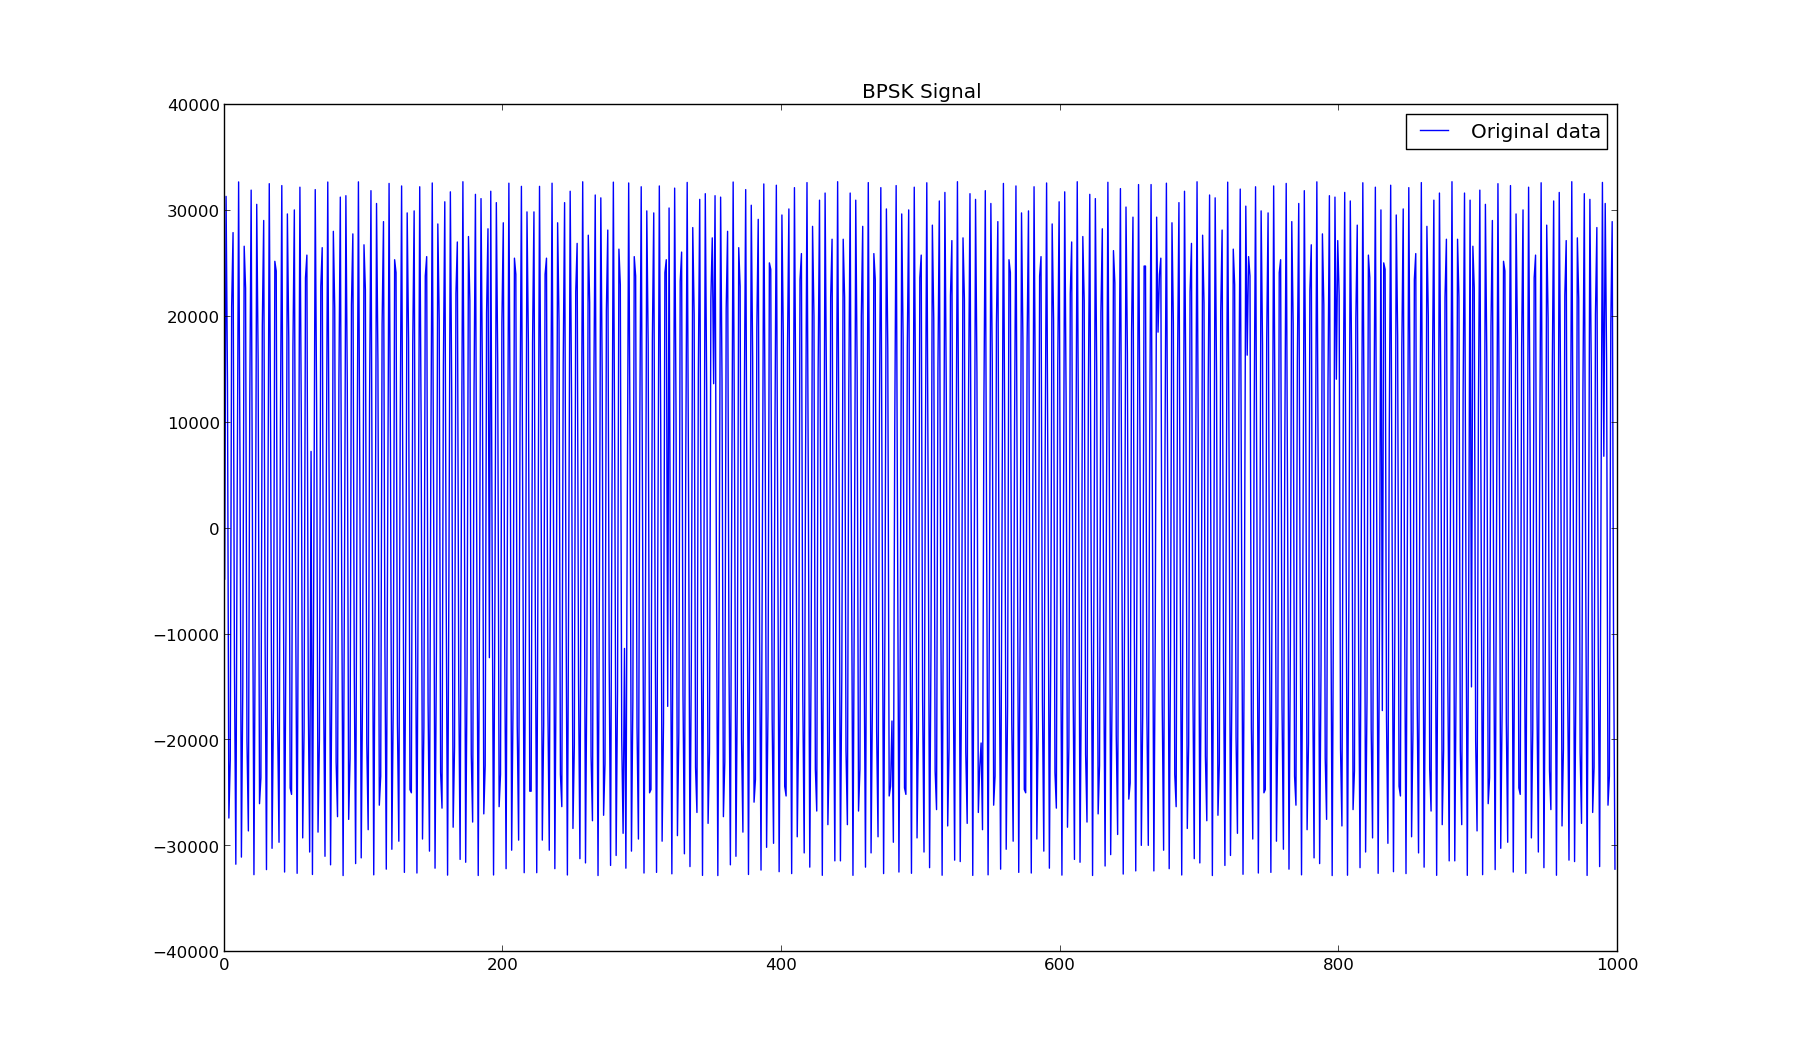
\includegraphics[width=0.5\textwidth]{wav_plot.png}
\caption{Plot of audio data}
\label{fig:WAV}
\end{figure}[h!]
\begin{figure}
\centering
  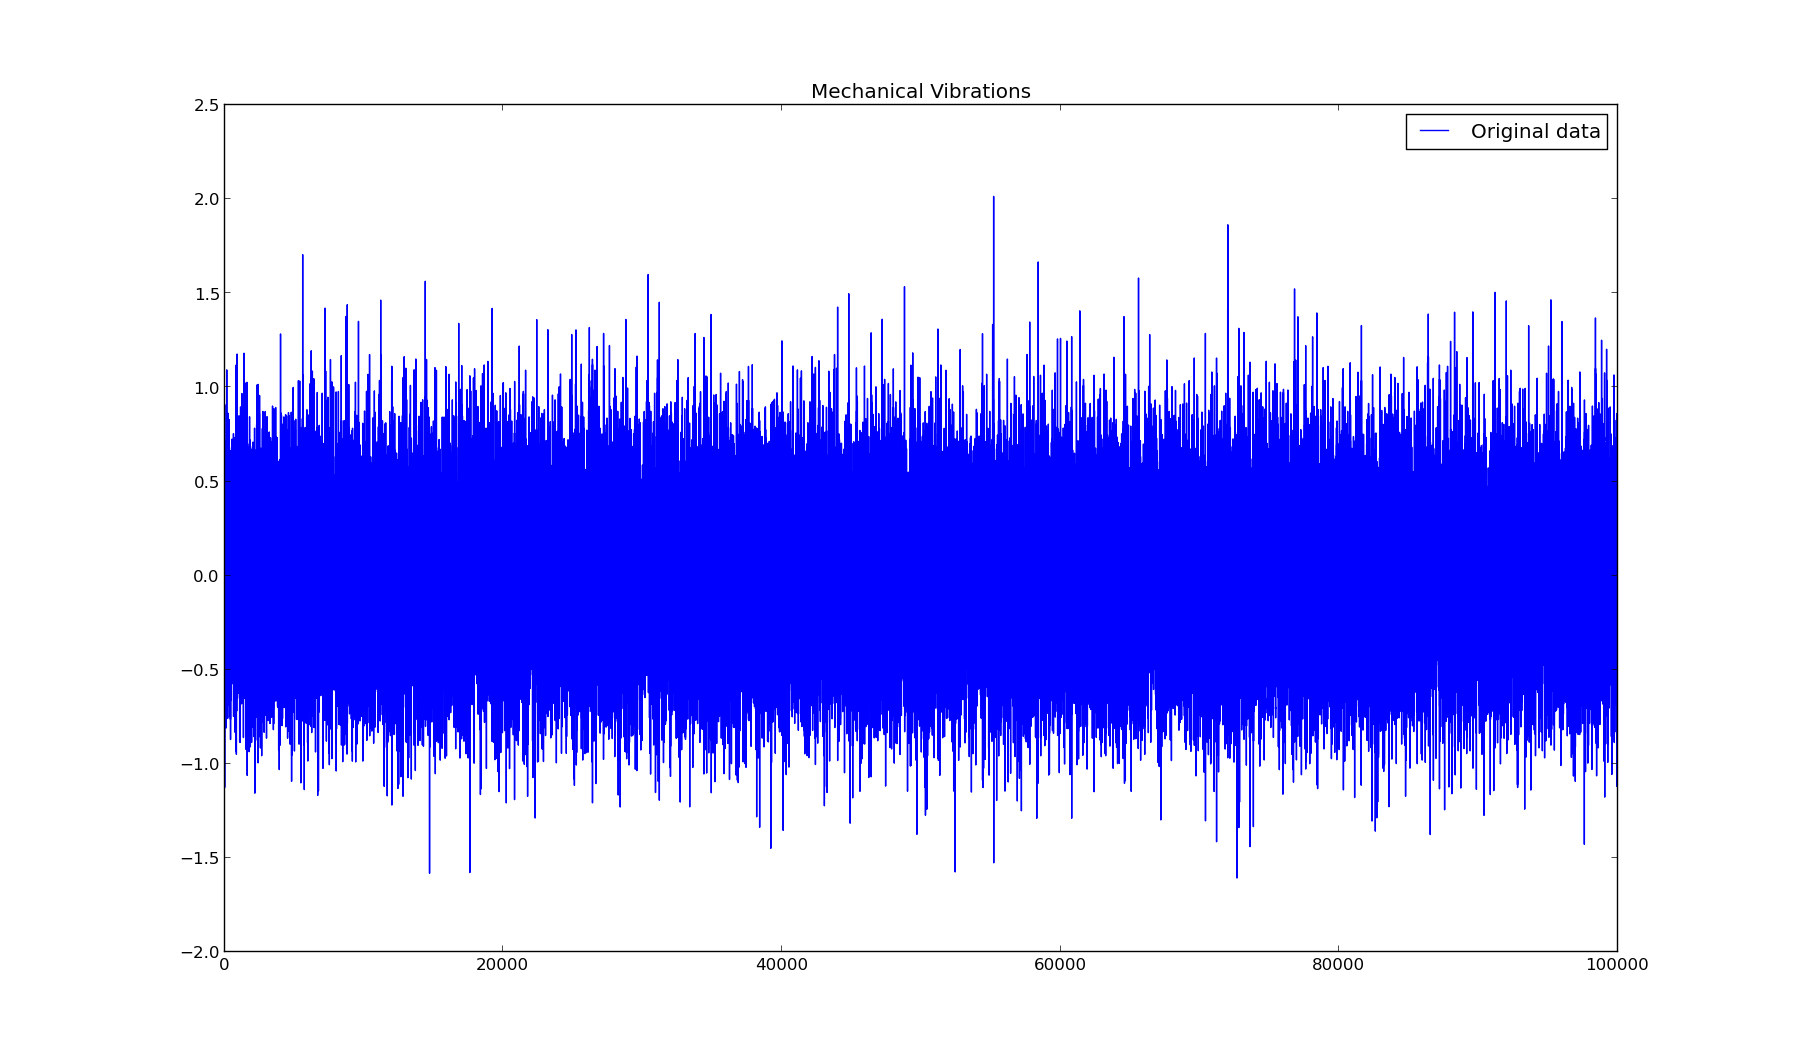
\includegraphics[width=0.5\textwidth]{matfile_plot.png}
\caption{Plot of mechanical data}
\label{fig:Mat}
\end{figure}
\begin{figure}[h!]
\centering
  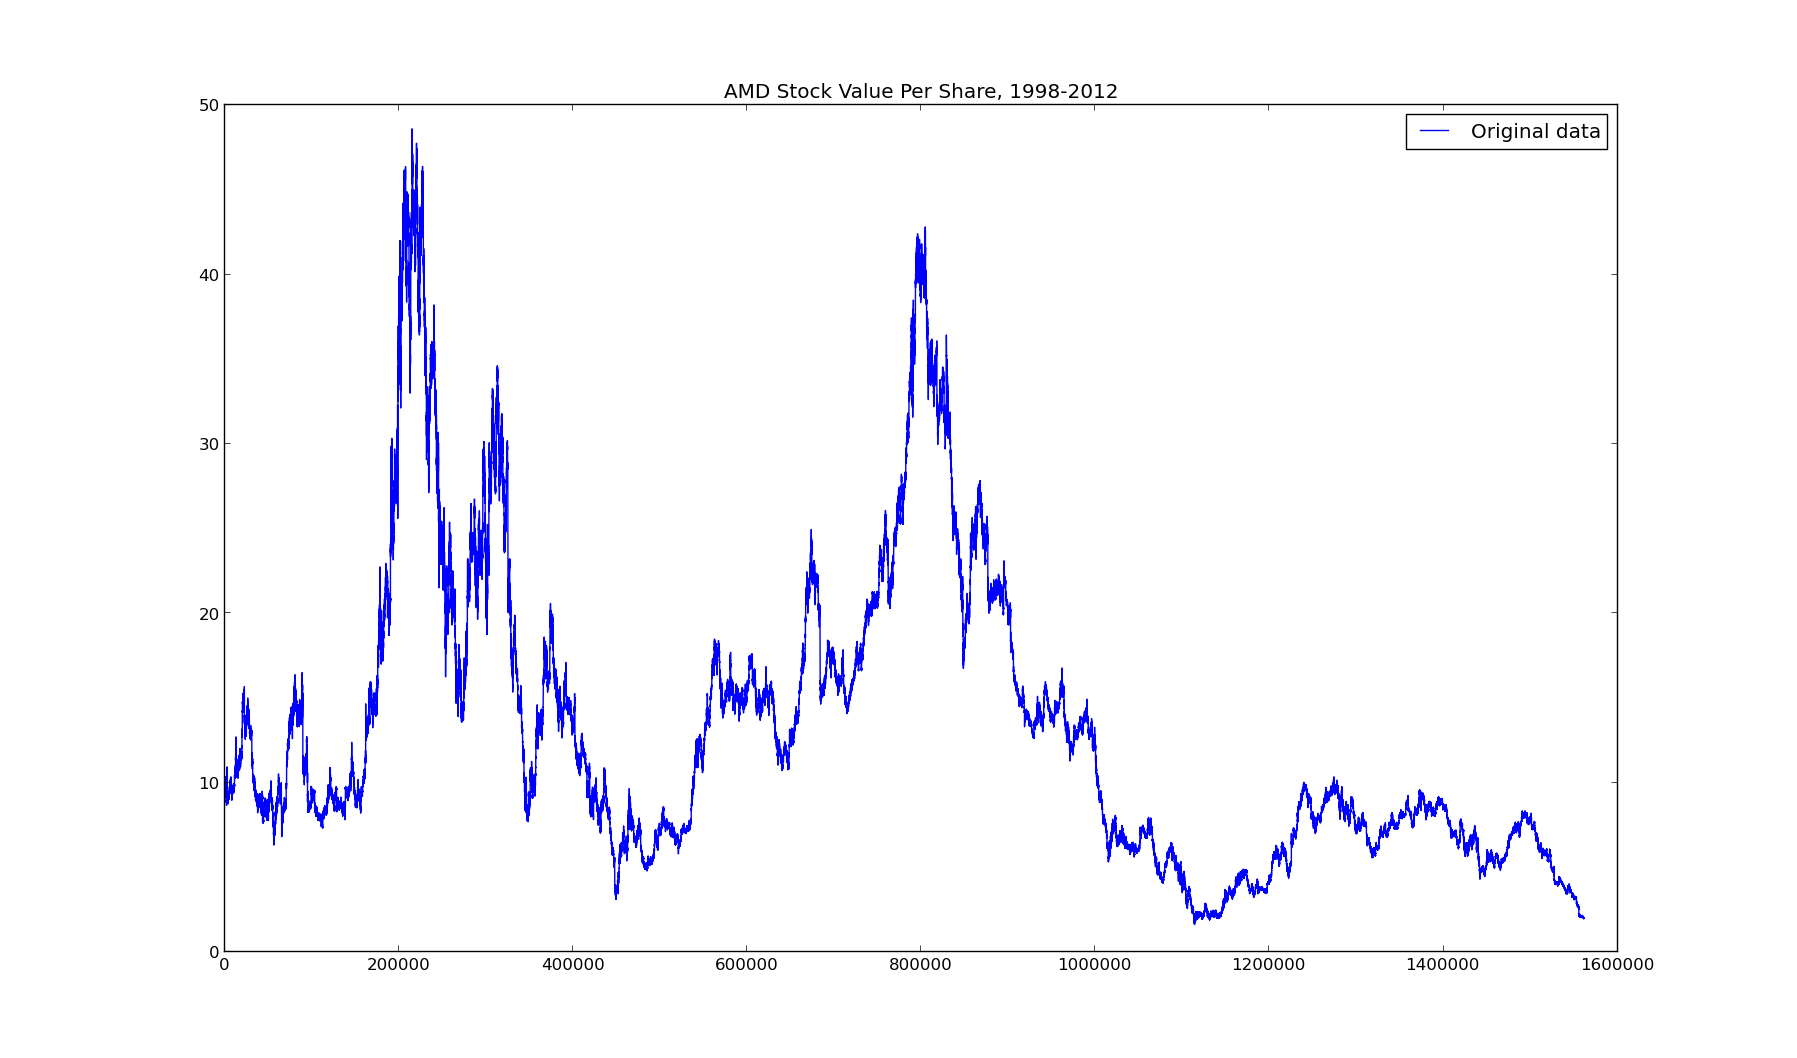
\includegraphics[width=0.5\textwidth]{stock_plot.png}
\caption{Plot of stock market data}
\label{fig:Stock}
\end{figure}

\section{Spectrogram}
The spectrogram is one of the most basic time-frequency analysis tools. It provides basic insight with minimal computational cost, but certain
types of data do not lend themselves well to this type of analysis.

\subsection{Formulation}
\begin{equation}
    Spectrogram(t,\omega) = \lvert STFT(t,\omega) \rvert ^2
    \label{eq:Spectrogram}
\end{equation}
The spectrogram is simply formulated in Eq. \ref{eq:Spectrogram}. \cite{DSPBook}

\begin{figure}[h!]
\centering
  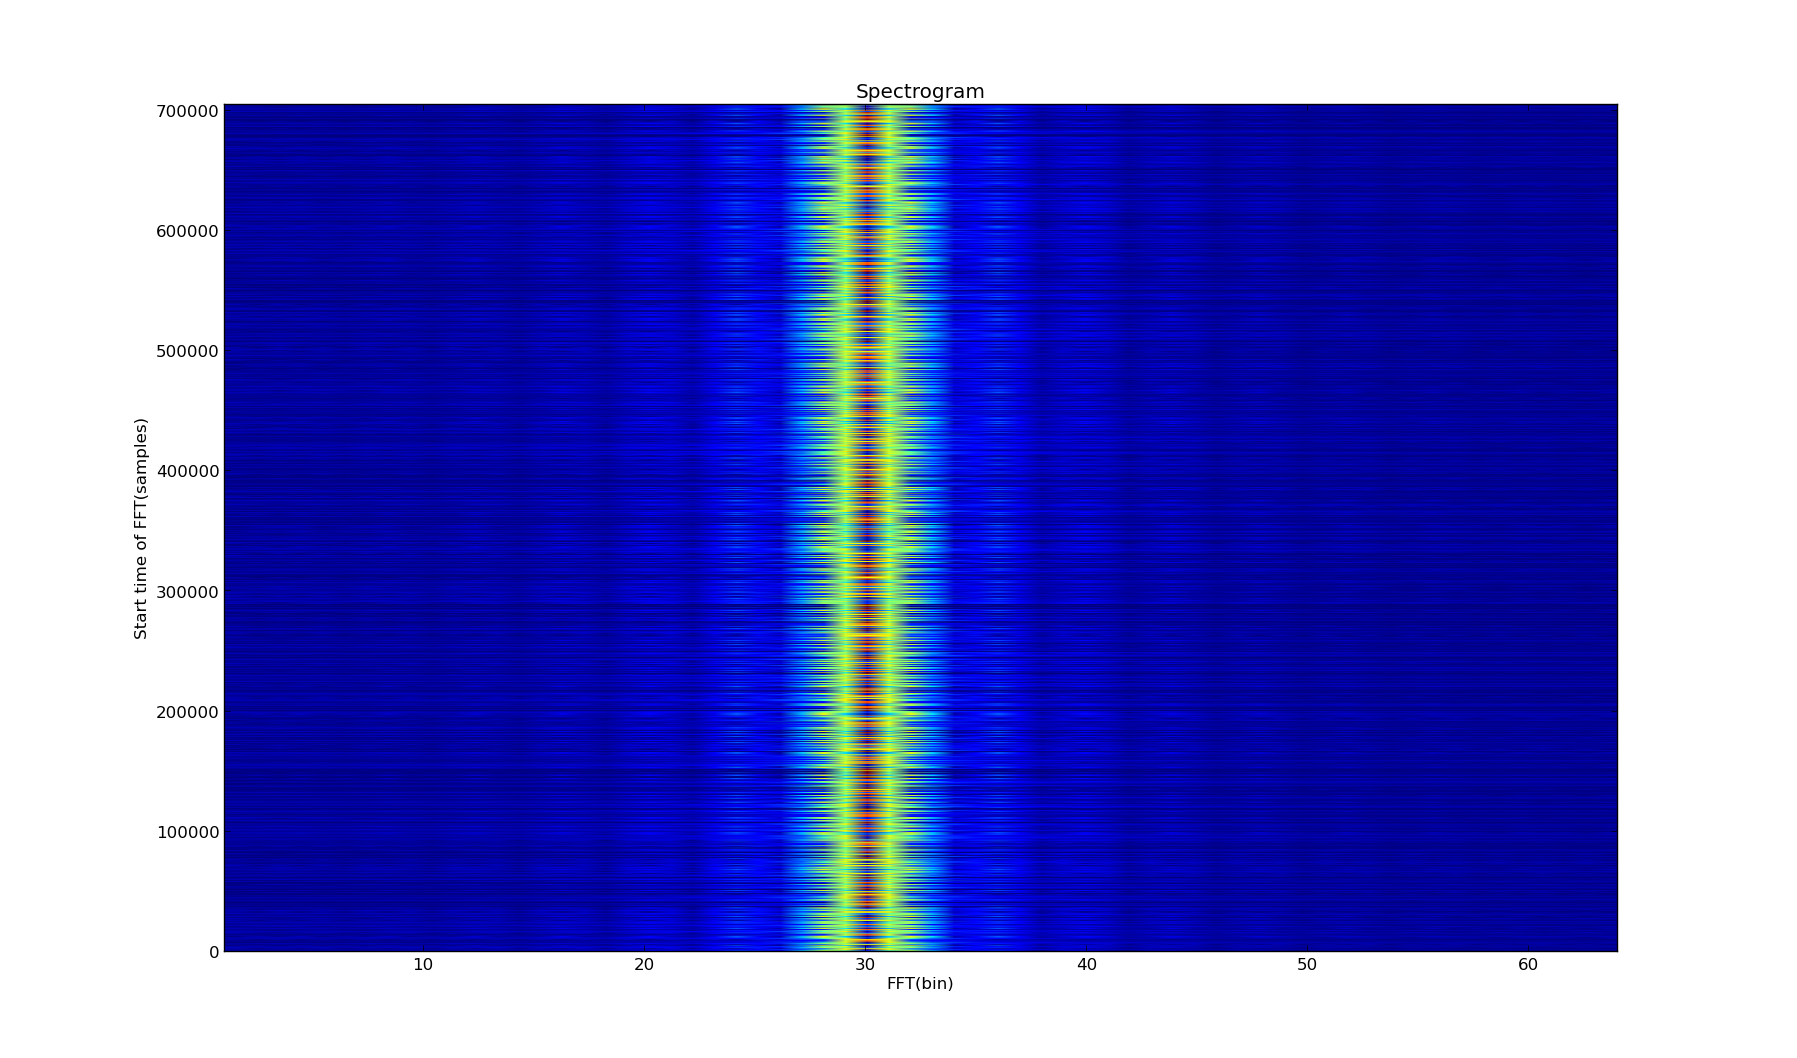
\includegraphics[width=0.5\textwidth]{wav_spectrogram_plot.png}
\caption{Spectrogram of audio data, NFFT$=128$,Window$=Hanning$}
\label{fig:WAVSpectrogram}
\end{figure}

\begin{figure}[h!]
\centering
  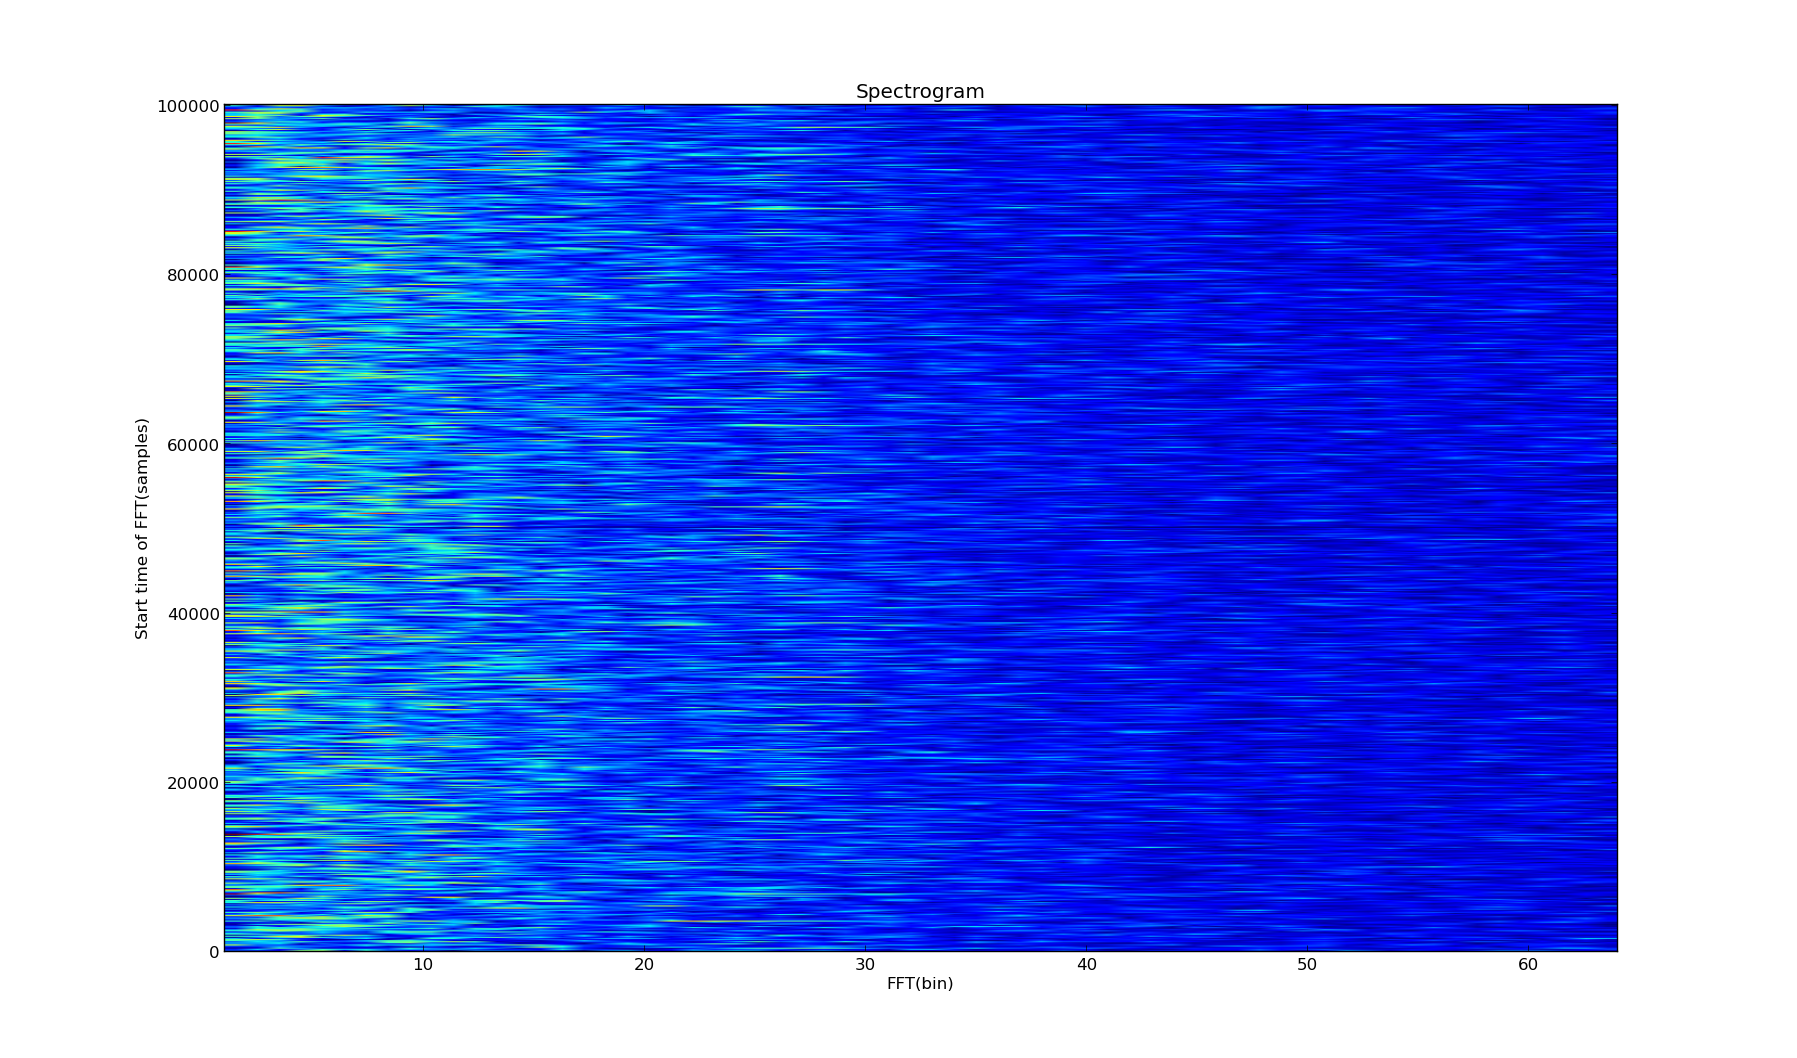
\includegraphics[width=0.5\textwidth]{matfile_spectrogram_plot.png}
\caption{Spectrogram of mechanical data, NFFT$=128$,Window$=Hanning$}
\label{fig:MatSpectrogram}
\end{figure}

\begin{figure}[h!]
\centering
  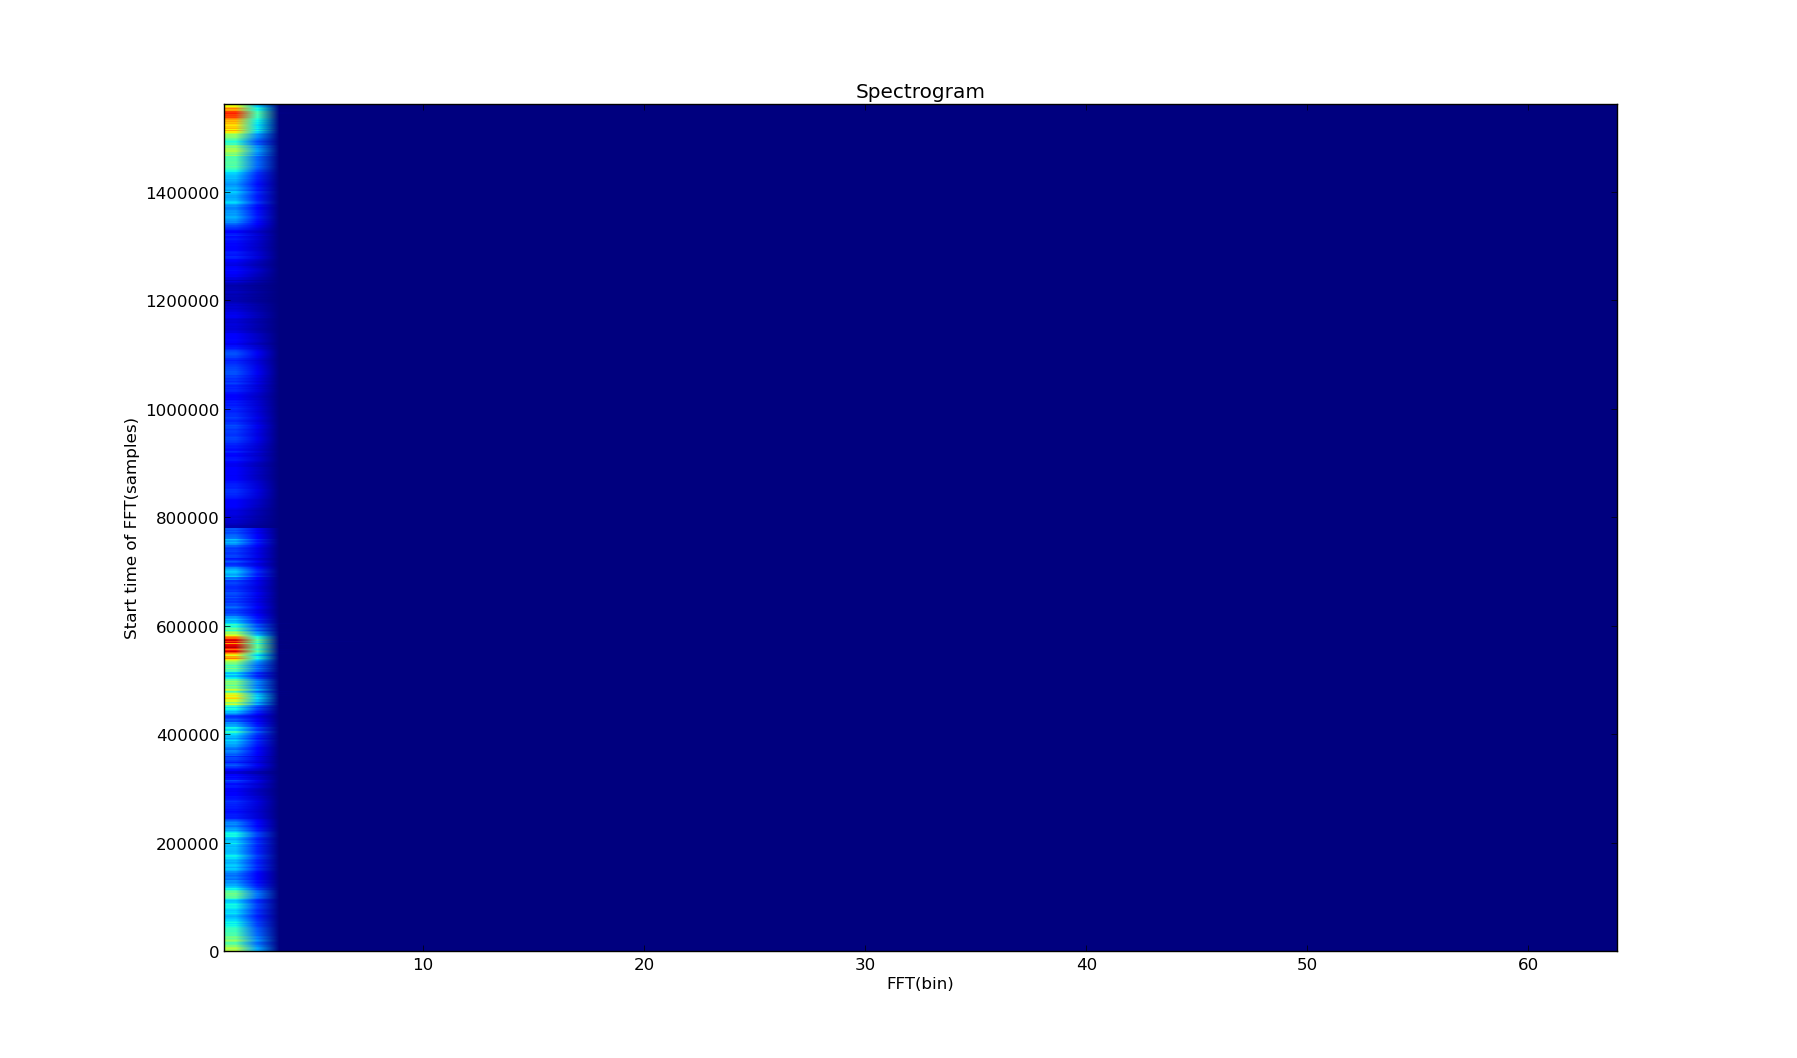
\includegraphics[width=0.5\textwidth]{stock_spectrogram_plot.png}
\caption{Spectrogram of stock market data, NFFT$=128$,Window$=Hanning$}
\label{fig:StockSpectrogram}
\end{figure}

\subsection{Usage}
The spectrogram has historically found its use in the analysis of communication signals and audio data. Due to its relatively moderate computational
intensity and simplicity of implementation, it is often the first technique used for time-frequency investigation of a dataset. As seen in Fig.
\ref{fig:WAVSpectrogram}, the spectrogram shows well the content of the audio data, which is a Binary Phase Shift Keyed (BPSK) signal. However, in Fig. 
\ref{fig:MatSpectrogram} and Fig. \ref{fig:StockSpectrogram}, there is little useful information to be gained from this view of the data.

One of the major downsides of this method is that the time-frequency tradeoff in FFT size is still 
critical. By choosing a small FFT size, it is easy to see the data has different frequency components over time, but it is difficult to see exactly
what frequencies those are. Choosing a large FFT size will give more accurate results, but sacrifice the desired time resolution.

\section{Wigner-Ville}
The Wigner-Ville distribution is a joint time-frequency distribution, which treats signals as being composed of basis functions which are stochastic 
processes with particular statistics, each taking on a different value at a particular time. Wigner-Ville analysis is used to attempt to see 
periodicity in the statistics of these basis functions. \cite{WignerPaper}

\subsection{Formulation}
\begin{equation}
    W_v(t,\omega) = \int x(t+\frac{\tau}{2})x^{*}(t-\frac{\tau}{2})e^{-j \omega t}d\tau
    \label{eq:WignerVille}
\end{equation}

\begin{figure}[h!]
\centering
  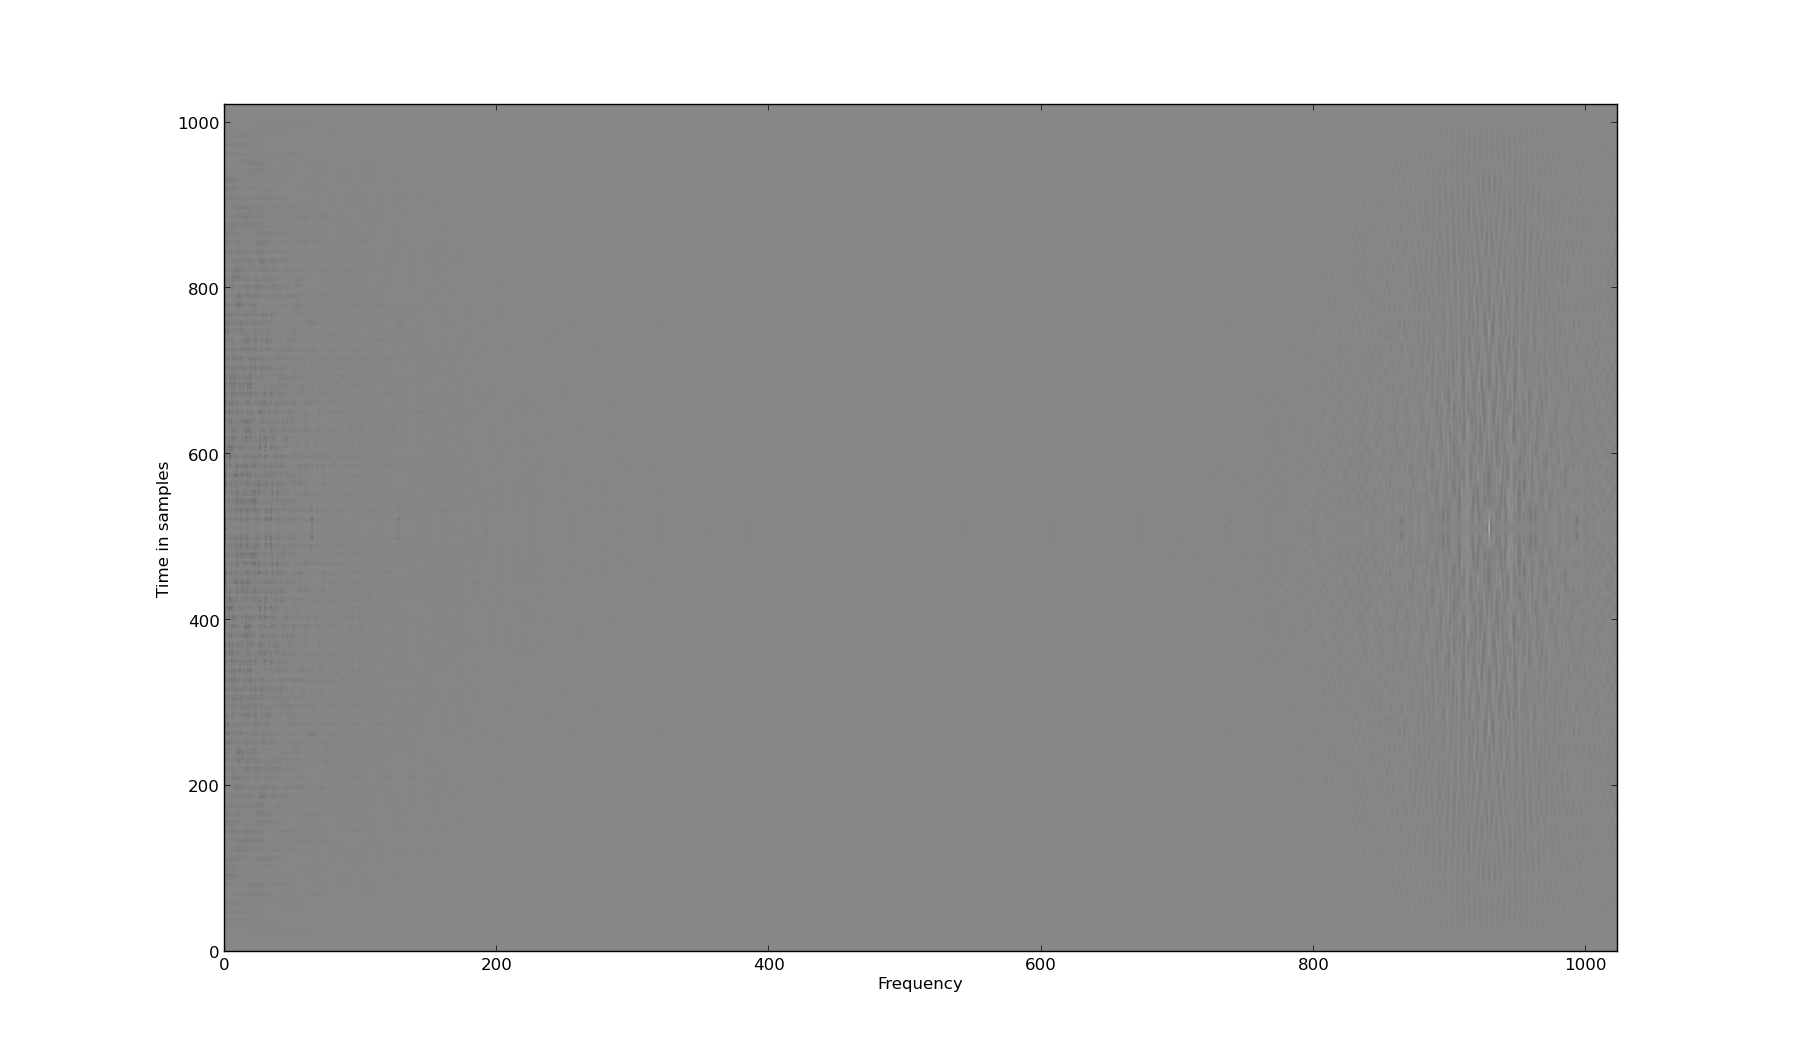
\includegraphics[width=0.5\textwidth]{wav_wigner_plot.png}
\caption{Wigner-Ville plot of audio data}
\label{fig:WAVWigner}
\end{figure}

\begin{figure}[h!]
\centering
  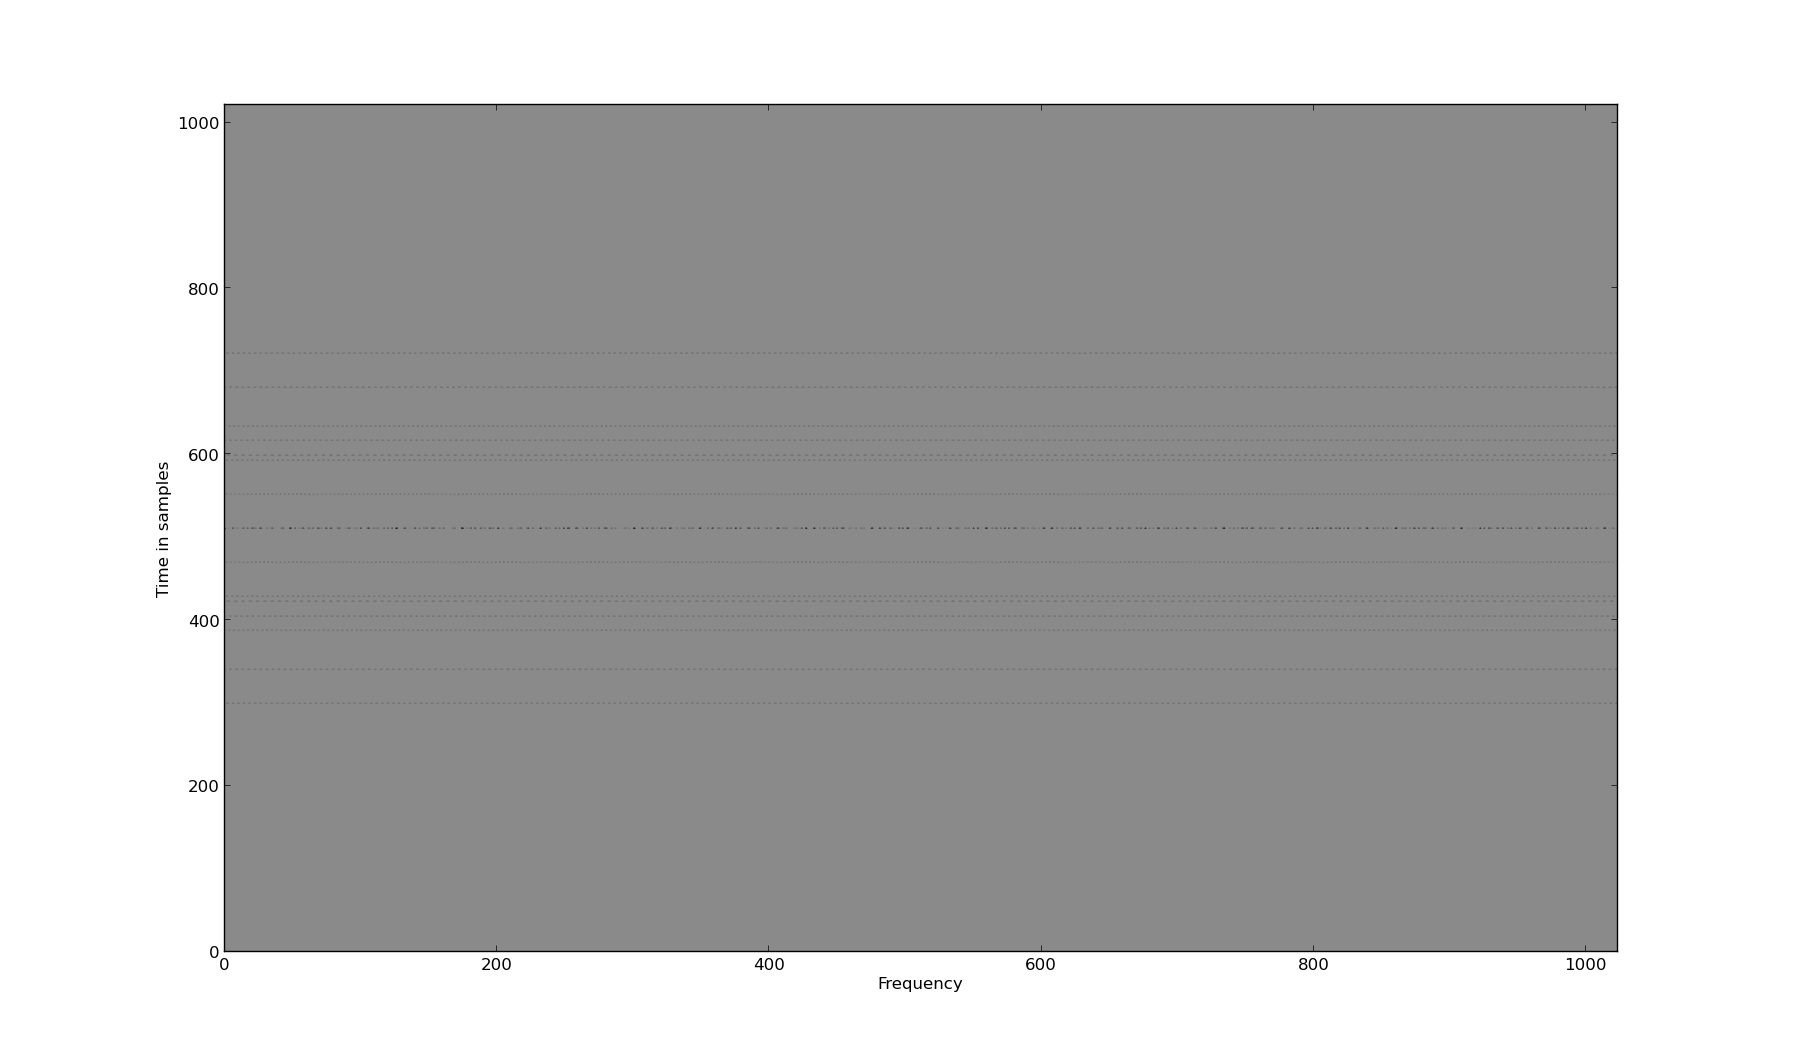
\includegraphics[width=0.5\textwidth]{matfile_wigner_plot.png}
\caption{Wigner-Ville plot of mechanical data}
\label{fig:MatWigner}
\end{figure}

\begin{figure}[h!]
\centering
  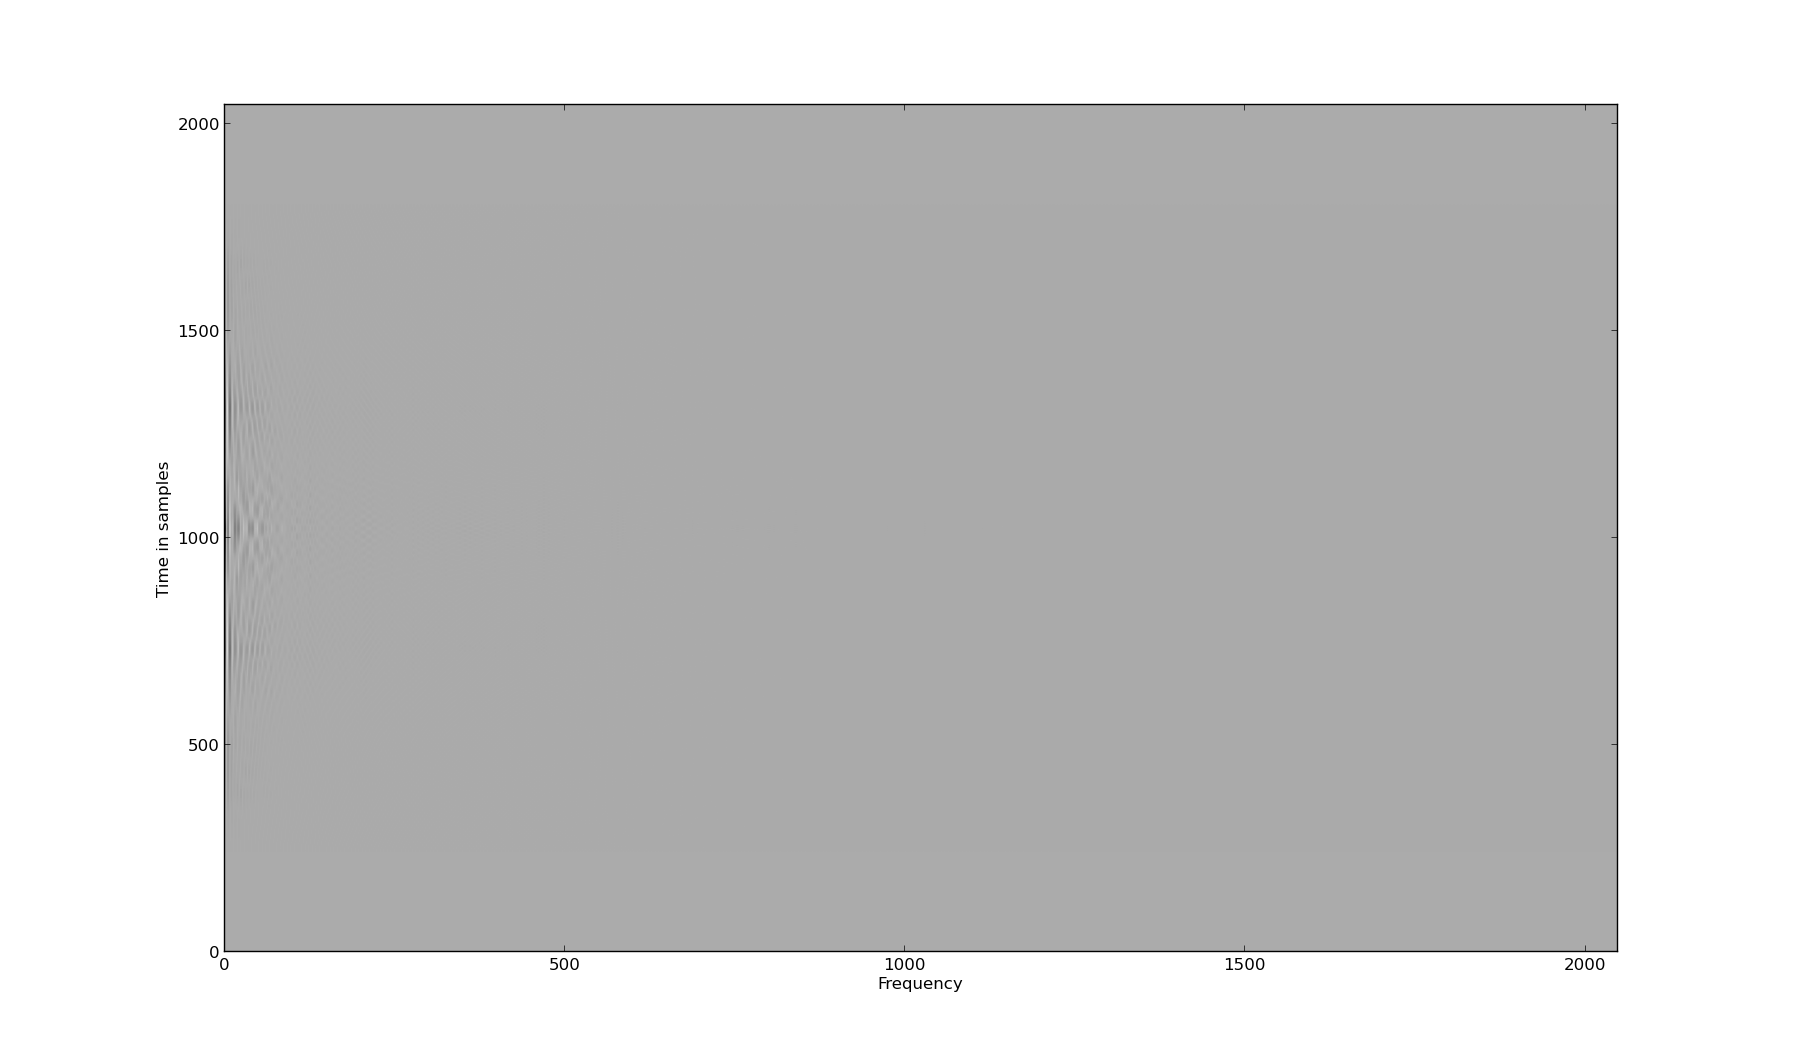
\includegraphics[width=0.5\textwidth]{stock_wigner_plot.png}
\caption{Wigner-Ville plot of stock market data}
\label{fig:StockWigner}
\end{figure}

\subsection{Usage}
As can be seen in Figures \ref{fig:WAVWigner}, \ref{fig:MatWigner}, there are some interesting features of the Wigner-Ville spectrum which
are not easily seen in the standard spectrogram. The mechanical data plot especially shows a clear pattern in both time and frequency, which 
relates to some component of the mechanical system being analyzed. The stock market data in Fig. \ref{fig:StockWigner} still has no particularly 
interesting features viewable in the Wigner-Ville spectrum. 

\section{Cyclic Coherence}
The third time-frequency analysis technique used was the cyclic coherence function (CCF), which is closely related to the spectral correlation function 
(SCF). These functions attempt to find cyclostationarity at different lag frequencies, typically defined as $\alpha$, between either
two different signals, or a signal with itself. Conceptually, this is similar to the relationship between correlation and autocorrelation. 

\subsection{Formulation}
\begin{equation}
    R_{xx}(\alpha,f) = \int R(t, \tau)e^{-j 2 \pi \alpha t}dt
\end{equation}
\begin{equation}
    S_{xx}^\alpha(\alpha,f) = \int R_{xx}(\tau,\alpha)e^{-j 2 \pi f \tau}d\tau 
\end{equation}
\begin{equation}
    \gamma_{xx}(f,\alpha) = \frac{S_{xx}(f,\alpha)}{S_{x0}(f+\beta \alpha)S_{x1}(f-\beta \alpha)}; \beta = \frac{1}{2}
\end{equation}

\begin{figure}[h!]
\centering
  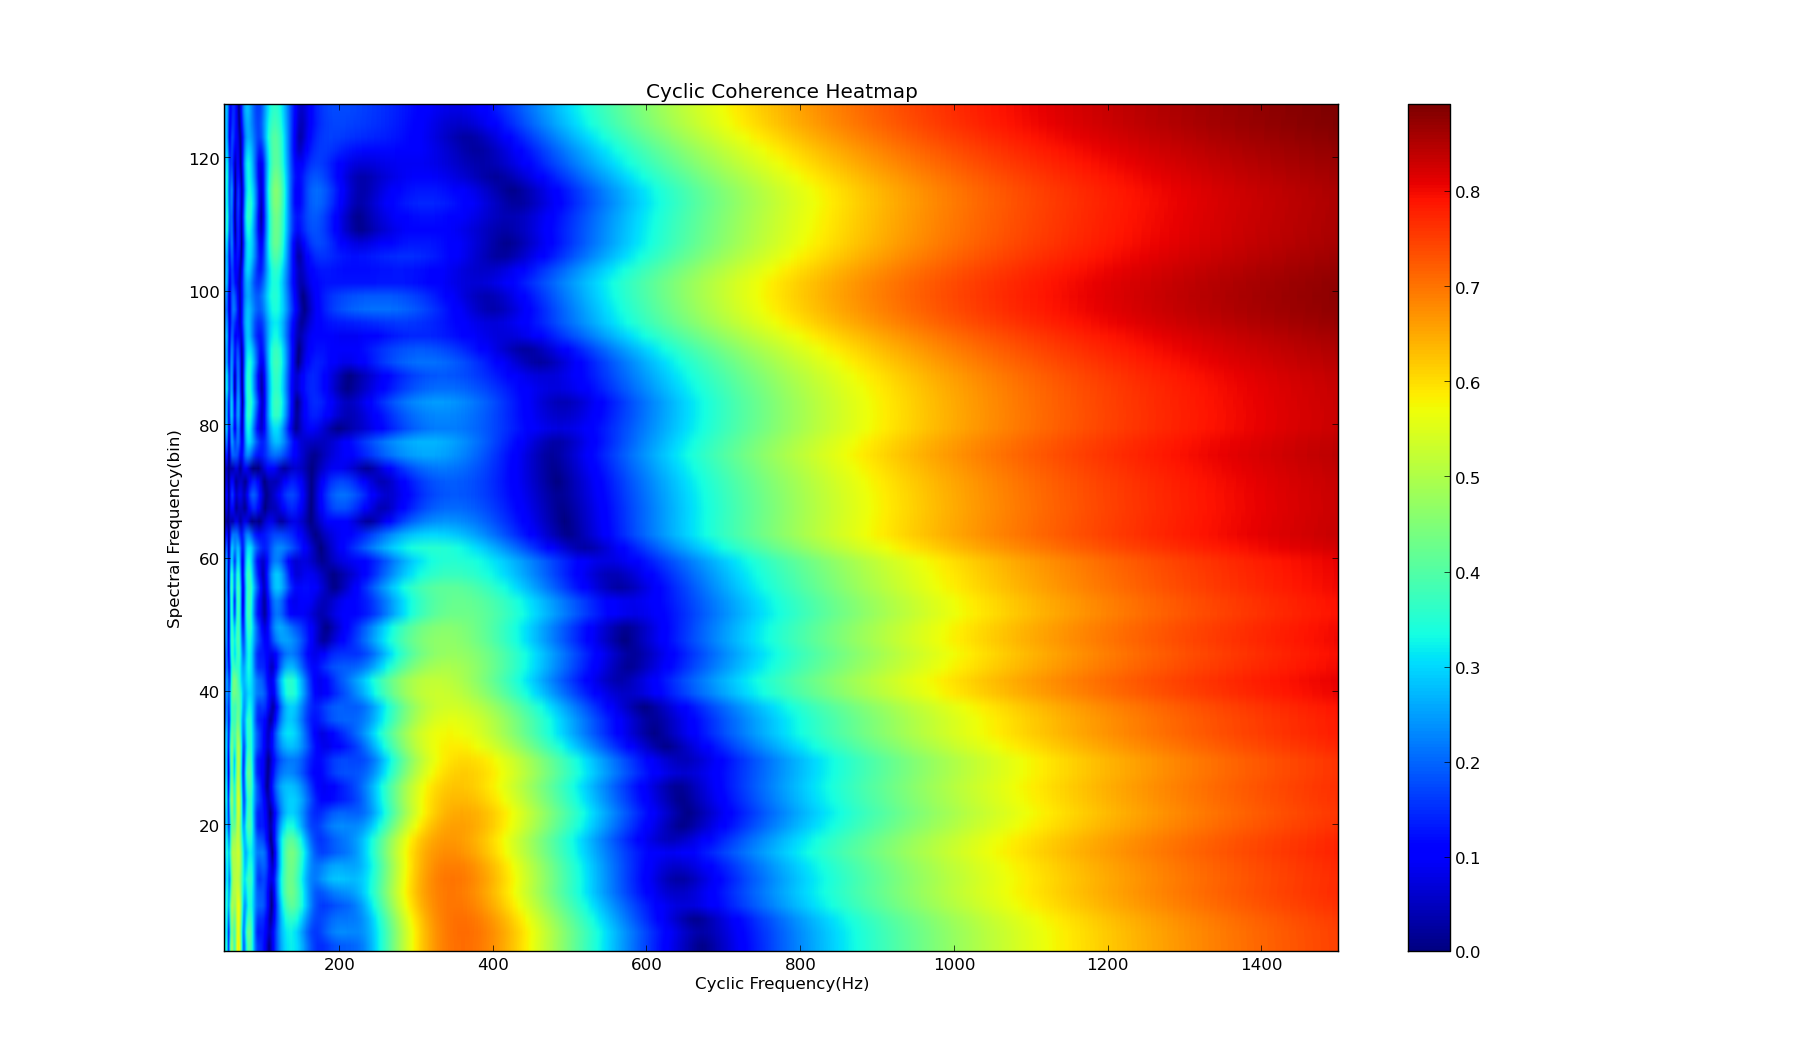
\includegraphics[width=0.5\textwidth]{wav_2d_plot.png}
\caption{Cyclic coherence plot of audio data}
\label{fig:WAVCoherence}
\end{figure}

\begin{figure}[h!]
\centering
  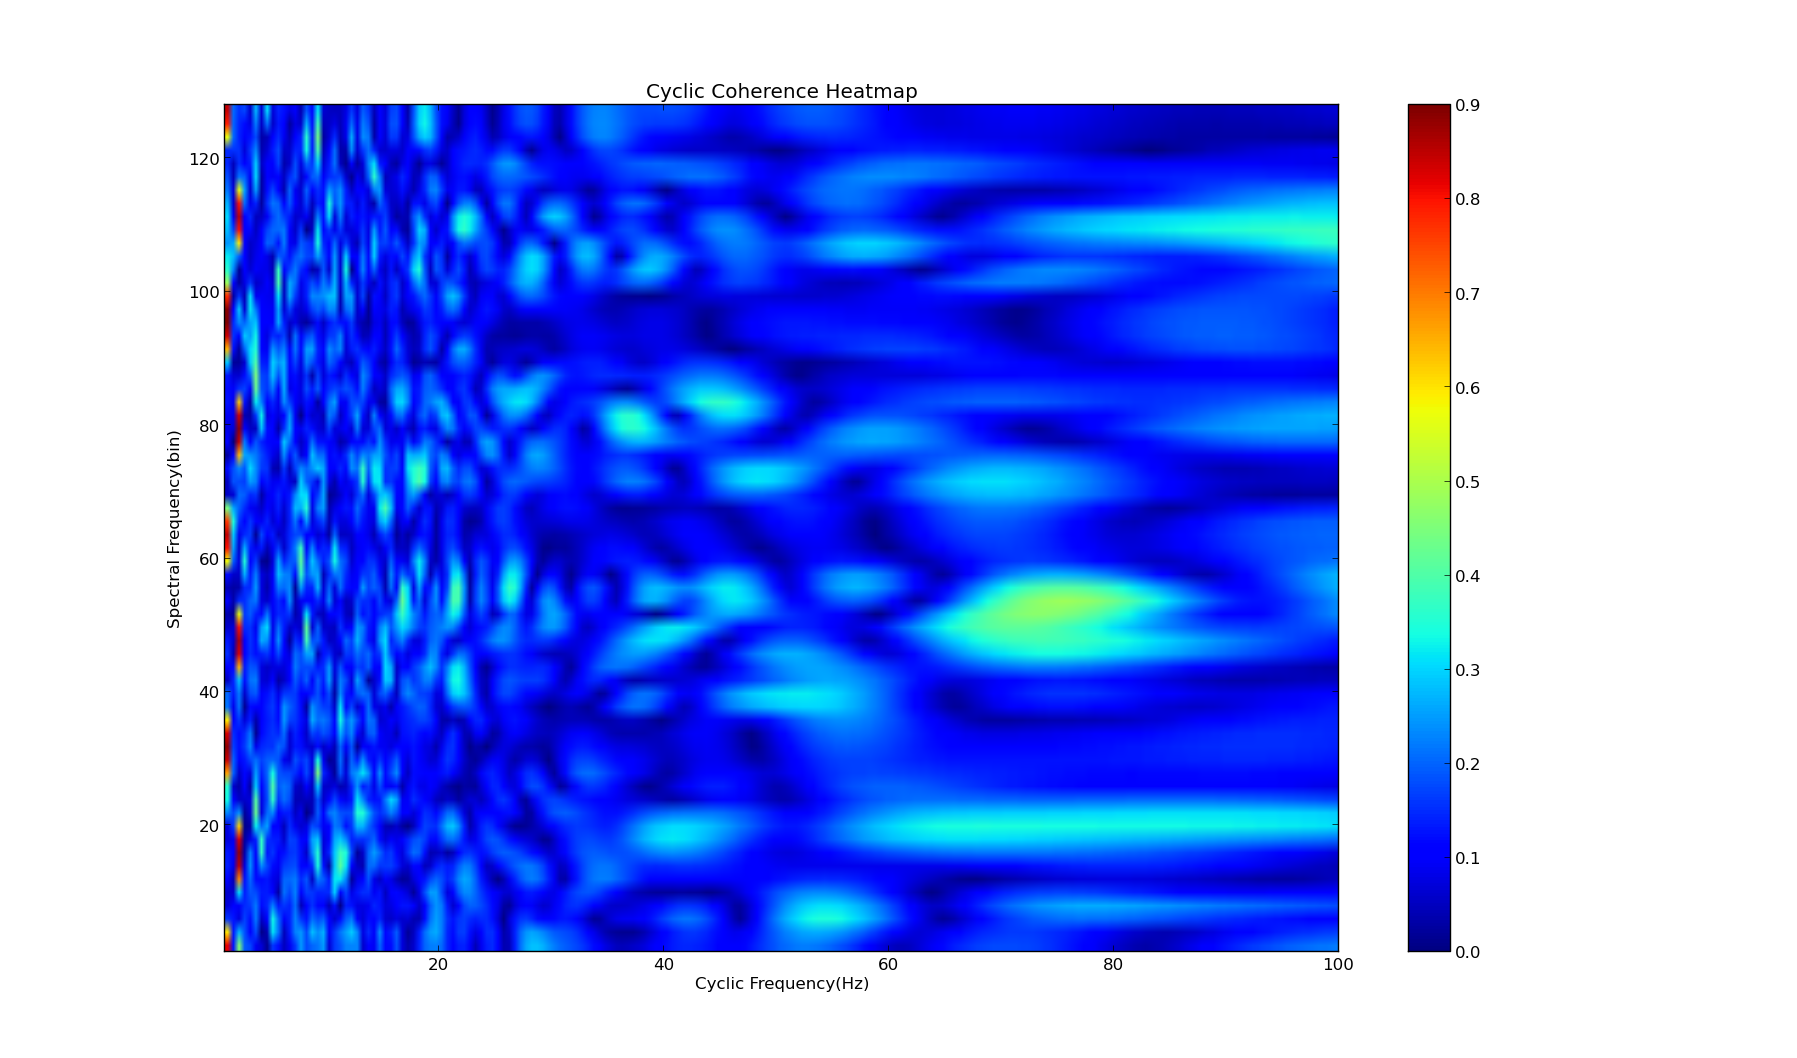
\includegraphics[width=0.5\textwidth]{matfile_2d_plot.png}
\caption{Cyclic coherence plot of mechanical data}
\label{fig:MatCoherence}
\end{figure}

\begin{figure}[h!]
\centering
  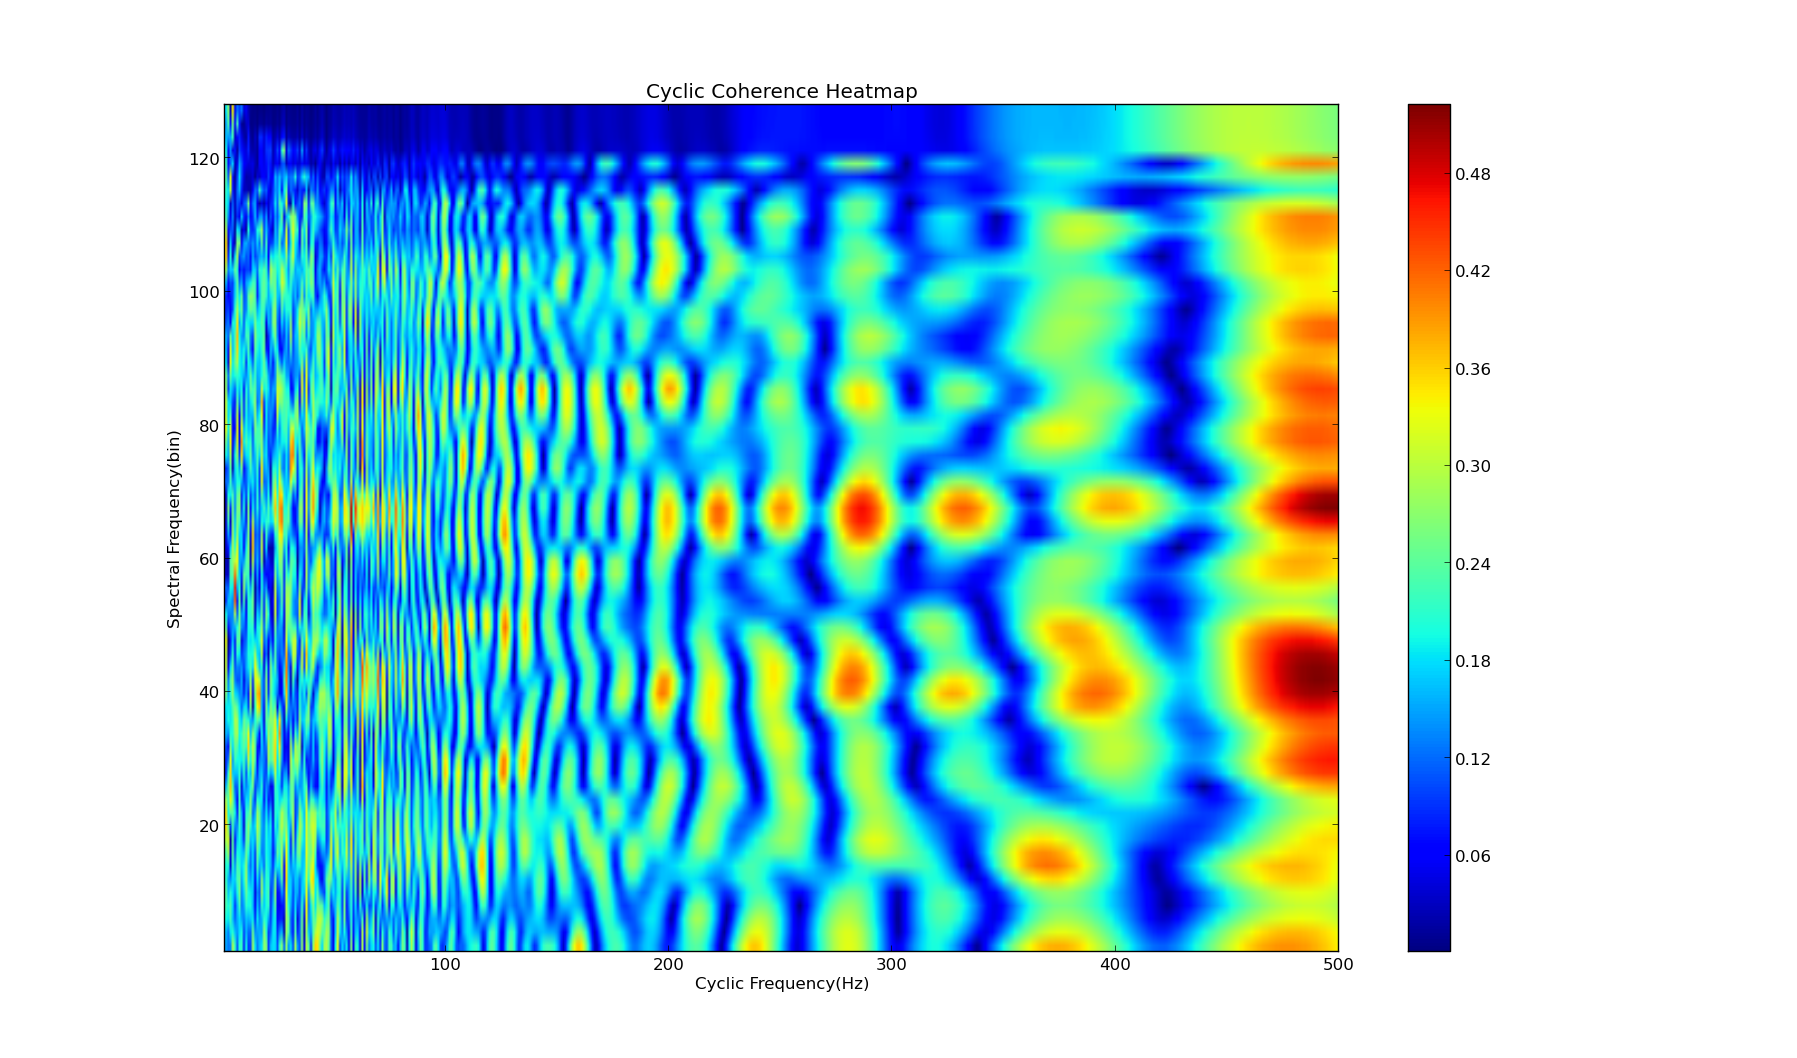
\includegraphics[width=0.5\textwidth]{stock_2d_plot_near.png}
\caption{Cyclic coherence plot of stock market data}
\label{fig:StockCoherence}
\end{figure}

\subsection{Usage}
As can be seen in Figure \ref{fig:StockCoherence}, there is some interesting cyclostationarity in the stock market data close to real-time. This
statistical periodicity could potentially be used to make decisions about whether to buy or sell a given stock at a certain time. A wider analysis will
be undertaken, in order to determine the usefulness and applicability of this technique over a wider diversity of stock types.

\section{Conclusion}
It appears that time-frequency analysis methods hold some promise. The cyclic coherence function appears to show some unique cyclostationarity in
the stock market data analyzed here, and may point the way to other related functions that may be useful. Further work will include employing the 
autoambiguity function (AAF), which is related to the cyclic coherence function, as well as the Choi-Williams distribution, which is related to the 
Wigner-Ville spectrum. There are also some interesting avenues exploring the spectral correlation function (SCF) of two different, seemingly unrelated 
stocks, in order to find hidden relationships between the two. The coherence function could potentially act as a weight to a sensor fusion technique, in 
order to combine information from multiple stocks into a single prediction. 

\begin{thebibliography}{1}
\bibitem{DSPBook}
A. Oppenheim, R. Schafer, and J. Buck, \emph{Discrete Time Signal Processing}, 2nd Edition. Prentice-Hall, 1999.

\bibitem{SignalData}
Francesco Pizzo, \emph{Simple examples of 16QAM and BPSK modulators}, bpsk.wav taken from mathworks.com, November 12, 2012. 
    
\bibitem{CyclicData}
J. Antoni, \emph{Dataset for Cyclic Spectral Analysis in Practice}, x.mat taken from Pack Cyclic Spectral Correlation.zip, http://www.utc.fr/~antoni/,
November 15, 2012.

\bibitem{StockData}
Kibot Free Data, AMD.txt taken from http://www.kibot.com/, November 20, 2012.

\bibitem{WignerPaper}
W. Martin, P. Flandrin, \emph{Wigner-Ville spectral analysis of nonstationary processes}, IEEE Transactions on Acoustics, Speech, and Signal Processing, 
Volume 33, Issue 6.

\bibitem{EarthquakePaper}
S. C. Bradford, J. Yang, T. Heaton, \emph{Variations in the Dynamic Properties of Structures: The Wigner-Ville Distribution}. April 18, 2006. 

\bibitem{HelicopterPaper}
E. Estupinan, P. White, C. Martin, \emph{A Cyclostationary Analysis Applied to Detection and Diagnosis of Faults in Helicopter Gearboxes}

\bibitem{CyclicPaper}
J. Antoni, \emph{Cyclic Spectral Analysis in Practice}, Mechanical Systems and Signal Processing, Volume 21, Issue 2 , February 2007.
\end{thebibliography}

% if you will not have a photo at all:
%\begin{IEEEbiographynophoto}{Kyle Kastner}
%Kyle is a graduate of Texas State University, B.S.E.E., who is currently pursuing an M.S.E.E at University of Texas-San Antonio.
%Research areas include powerline communications, cognitive radio, music classification and radiolocation techniques.
%He is curently employed by Southwest Research Institute, Division 16. 
%\end{IEEEbiographynophoto}

%\begin{IEEEbiographynophoto}{Johanna Hansen}
%Johanna Hansen works at Southwest Research Institute, Division 10.
%\end{IEEEbiographynophoto}

% You can push biographies down or up by placing
% a \vfill before or after them. The appropriate
% use of \vfill depends on what kind of text is
% on the last page and whether or not the columns
% are being equalized.

%\vfill

% Can be used to pull up biographies so that the bottom of the last one
% is flush with the other column.
%\enlargethispage{-5in}

% that's all folks
\end{document}


